\documentclass[a4paper,11pt]{article}
\usepackage{amsmath}
\usepackage{amssymb}
\usepackage{fullpage}
\usepackage{rotating}
\usepackage{tikz} \usetikzlibrary{trees}

\newcommand{\AnyCond}[1]{\text{Any}(#1)}
\newcommand{\BoundedCond}[1]{\text{Bounded}(#1)}
\newcommand{\Constraint}[1]{\textsc{#1}}
\newcommand{\DepProps}{\textit{DepProps}}
\newcommand{\Distinct}{\Constraint{Distinct}}
\newcommand{\Element}{\Constraint{Element}}
\newcommand{\Failed}{\text{Failed}}
\newcommand{\FailedCond}[1]{\text{Failed}(#1)}
\newcommand{\FixedCond}[1]{\text{Fixed}(#1)}
\newcommand{\Fixpoint}{\text{AtFixpt}}
\newcommand{\NoneCond}[1]{\text{None}(#1)}
\newcommand{\Gecode}{\textit{Gecode}}
\newcommand{\GIST}{\textit{GIST}}
\newcommand{\Propagate}{\text{Propagate}}
\newcommand{\PropConds}[1]{\text{PropConds}(#1)}
\newcommand{\Sequence}[1]{\left[#1\right]}
\newcommand{\Set}[1]{\left\{#1\right\}}
\newcommand{\Subsumed}{\text{Subsumed}}
\newcommand{\Tuple}[1]{\left\langle#1\right\rangle}
\newcommand{\Unknown}{\text{Unknown}}

%Min commandon
\newcommand{\Tdots}{\, .\, .\,}

%\pagestyle{empty}

\renewcommand{\thesubsection}{\Alph{subsection}}
\renewcommand{\thesubsubsection}{\Alph{subsection}.\alph{subsubsection}}

\title{\textbf{Low-Level Parallel Programming \\
    Uppsala University -- Spring 2015 \\
    Report for Lab~1
    by Team~21  % replace t by your team number
  }
}

\author{Markus Palacios, Jonathan Sharyari, Peng Sun} % replace by your name(s)

%\date{Month Day, Year}
\date{\today}


\begin{document}
\maketitle

\section{Questions}
\begin{description}
    \item[A] \textbf{What kind of parallelism is exposed with your code refactorization?}
 \hfill \\ 
 
    \item[B] \textbf{Give a short summary of similarities between SIMD and CUDA} \hfill \\Both techniques are the most efficient for data parallelism; they are able to execute the same instructions on multiple sets of data in parallel. 
    
    \item[C] \textbf{Which parallelization has been most beneficial in these two labs? Support your
case using plotted timing measurements} \hfill \\When comparing the techniques used in lab 1 with the ones used in this lab, these techniques prove to lower the time complexity. Tests show that CUDA(and SIMD?) tend to have a linear time complexity. 

    \item[D] \textbf{What kind of code transformations were required for this lab, and why were they
needed?} \hfill \\in $ped_agent.h$, the agent's x,y and z-values were stored in a struct. This made it hard for us to utilize parallelization in SIMD, as we'd always have to write each value to an array. We chose to instead instantiate arrays that hold each of the agents' x, y and z values, for faster access of the values in CUDA and SIMD. 

Neither CUDA nor SIMD uses the pre-existent functions Go() and whereToGo(), and instead calculates these values by themselves. 

    \item[E] \textbf{Compare the effort required for each of the four parallelization techniques. Would
it have made a difference if you had to build the program from scratch, instead
of using given code?} \hfill \\ Yes. Since we've been forced to make major changes to how the program is implemented, it would have been easier to simply adapt the algorithm to fit our parallelization techniques instead of rewriting the existing one. 
\end{description}

\section{How to run}
Without an argument specifying the type of parallelism, the serial version is used, whereas --pthreads and --openmp activates pthreads and openmp respectively (in case both are set, the last occurance will be dominating). The number of threads can in both cases be set by --np X. The value of X is ignored in the serial case.
\begin{description}
    \item[Serial] ./demo
    \item[OpenMP] ./demo --openmp
    \item[Pthreads] ./demo --pthreads --np 4
\end{description}
   
\subsection{Experiments}
Our experiments were run under Ubuntu Linux ~14.04 (64~bit) on an
Intel Core~i3~550 of 3.2~GHz with an 4~MB L2 cache and a 4~GB RAM.



\section*{Intellectual Property}
We certify that this report is solely produced by us, except where
explicitly stated otherwise and clearly referenced, and that we can
individually explain any part of it at the moment of submitting this
report.


\begin{figure}[h!]
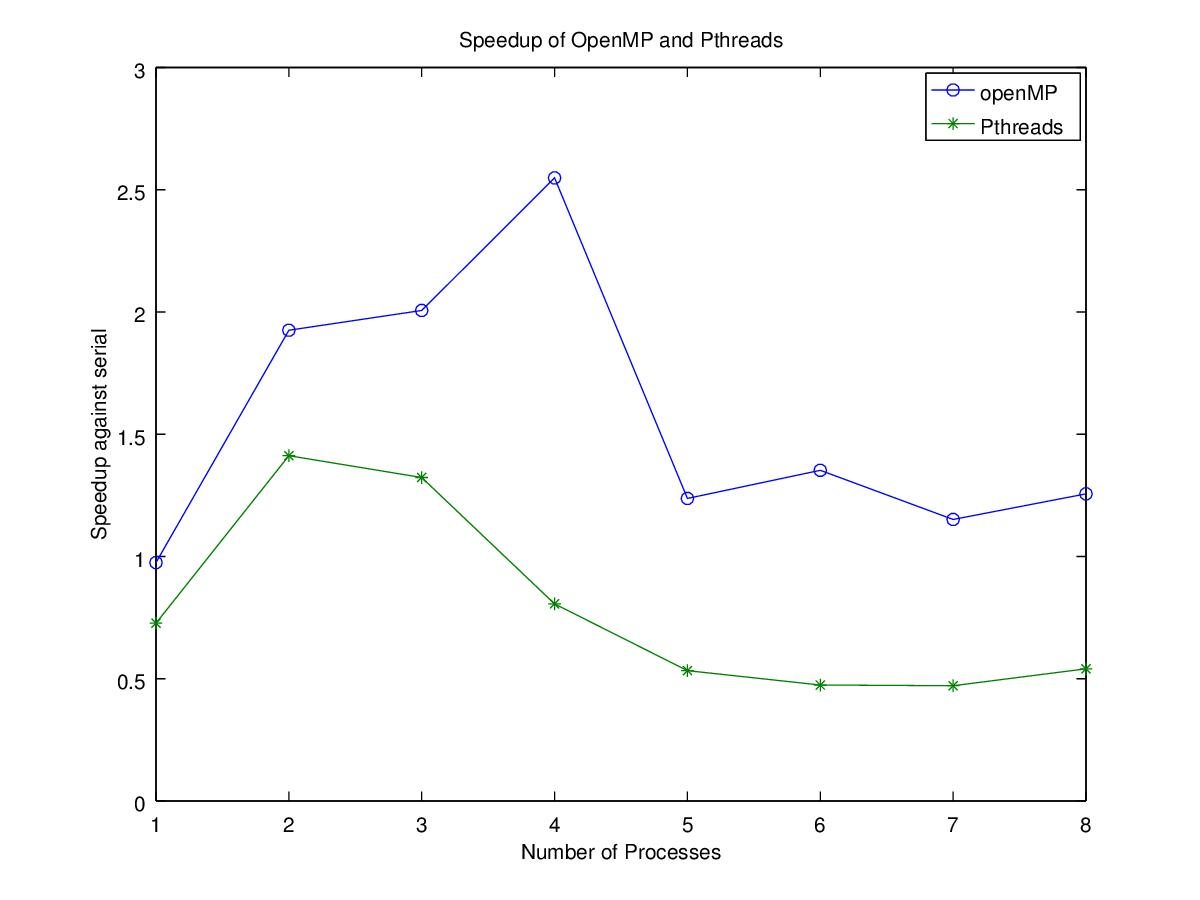
\includegraphics[width=\textwidth]{graph.jpg}
\caption{Graph showing the speedup of openmp and pthreads for 1 to 8 threads.}
\label{figure1}
\end{figure}



\end{document}
